% 2023 全国甲卷文科 18：三棱柱 ABC-A1B1C1
% 源图点位与遮挡：底面 AC、CB 及棱 CC1 被遮挡；题设线段 A1C 也画为虚线。
% 可见棱和题设线段 A1B 为实线。源图没有直角、长度或等长标记。
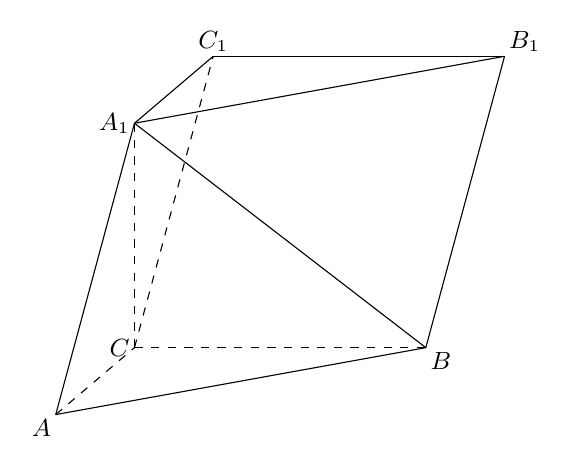
\begin{tikzpicture}[font=\small, line width=0.4pt,
  every node/.style={inner sep=1.5pt}]
  % 图纸坐标只用于复现原卷投影；上下两个三角形保持同一平移向量。
  \coordinate (A)  at (0,0);
  \coordinate (C)  at (1.00,0.85);
  \coordinate (B)  at (4.70,0.85);
  \coordinate (A1) at (1.00,3.70);
  \coordinate (C1) at (2.00,4.55);
  \coordinate (B1) at (5.70,4.55);

  % 遮挡棱及题设虚线先画，保证交叉处的可见实线在前。
  \draw[dashed] (A) -- (C);
  \draw[dashed] (C) -- (B);
  \draw[dashed] (C) -- (C1);
  \draw[dashed] (A1) -- (C);

  % 可见棱
  \draw (A) -- (B);
  \draw (A) -- (A1);
  \draw (A1) -- (C1);
  \draw (C1) -- (B1);
  \draw (B1) -- (B);
  \draw (A1) -- (B1);

  % 题面明确画出的线段 A1B
  \draw (A1) -- (B);

  % 顶点标注
  \node[anchor=north east] at (A)  {$A$};
  \node[anchor=east]       at (C)  {$C$};
  \node[anchor=north west] at (B)  {$B$};
  \node[anchor=east]       at (A1) {$A_1$};
  \node[anchor=south]      at (C1) {$C_1$};
  \node[anchor=south west] at (B1) {$B_1$};
\end{tikzpicture}
